\documentclass[11pt, oneside]{article}   	% use "amsart" instead of "article" for AMSLaTeX format
\usepackage{geometry}                		% See geometry.pdf to learn the layout options. There are lots.
\geometry{letterpaper}                   		% ... or a4paper or a5paper or ... 
%\geometry{landscape}                		% Activate for for rotated page geometry
%\usepackage[parfill]{parskip}    		% Activate to begin paragraphs with an empty line rather than an indent
\usepackage{graphicx}				% Use pdf, png, jpg, or eps� with pdflatex; use eps in DVI mode
								% TeX will automatically convert eps --> pdf in pdflatex		
\usepackage{amssymb}
\usepackage{amsmath}
\usepackage{parskip}
\usepackage{color}


\title{Theory}
%\author{The Author}
%\section{}
% \subsection*{R code}
\date{}							% Activate to display a given date or no date

\graphicspath{{/Users/telliott_admin/Dropbox/Tex/png/}}
% \begin{center} 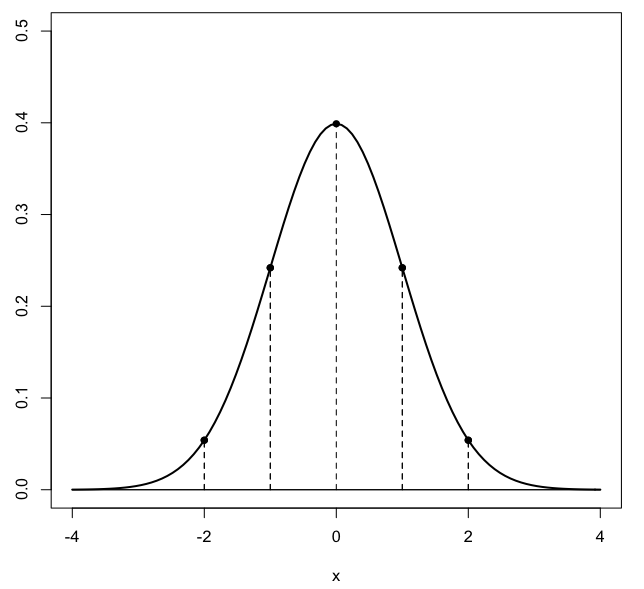
\includegraphics [scale=0.4] {gauss3.png} \end{center}

\begin{document}
\maketitle
\Large
A simple approach to calculus, which one might call the engineer's approach, consists of just using standard rules to calculate derivatives, and keeping track of the answers so that we can reverse the process to integrate.  In this way we can solve a wide variety of interesting and practical problems.

We "think of $dx$ as a little bit of $x$, and $dt$ as a little bit of $t$" and we work with the ratio $dx/dt$ as these quantities become very small.  We do not insist that $dt$ (or $dx$) become zero, as long as they become so small that a further reduction in size does not change the ratio appreciably.

Calculus was used in this way by mathematicians for more than a hundred years, with great success, and this general approach was still taught to most students until early in the 20th century.

A new method then entered, a more sophisticated one in which limits are emphasized, becoming ever more complicated as the discussion becomes more rigorous.  We can think of this as the "delta and epsilon" approach.  

In addition to rigor, mathematicians also want to know what to do with functions that are not as well-behaved as $f(x) = x^2$.  Some of these may be termed "pathological" functions, and they are mainly of theoretical interest.

\subsection*{infinity}
We introduce  the concept of infinity as representing something very large.  










\subsection*{}
\vspace{10mm}

\subsection*{Differentiability}

A function is differentiable at a point $x=a$ if the derivative is defined at that point, that is if this limit

\[ f'(x) = \lim_{h \to 0} \frac{f(x+h) - f(x)}{h} \]

is defined at $x=a$, that is, if

\[ \lim_{h \to 0} \frac{f(a+h) - f(a)}{h} \]
exists.  And this must be true as  $h \to 0-$ as well as $h \to 0+$.

So for example

\[ f(x) = \ln x \]
\[ f'(x) = \frac{1}{x} \]

In the above example, $f(x)$ is differentiable everywhere, except at $x=0$.

\subsection*{Continuity}

Continuity has an intuitive definition:  we should be able to graph the function \emph{without lifting pencil from paper}.  Basically, we require that for a function to be continuous at a point $x=a$, if we move $x$ away from $a$ by a little bit (either higher or lower), then $f(x)$ should not change from $f(a)$ by too much.  

A formal definition uses the apparatus of limits:  epsilons and deltas.  We implement this backwards (as usual) by specifying how large we allow the change in $f(x)$ to be, call it $\epsilon$.  Then if we can find $\delta$, a change in $x$, such that 

\[ | f(x \pm \delta) - f(x) | < \epsilon \]

for \emph{any} $\epsilon$, we are good.

\begin{center} 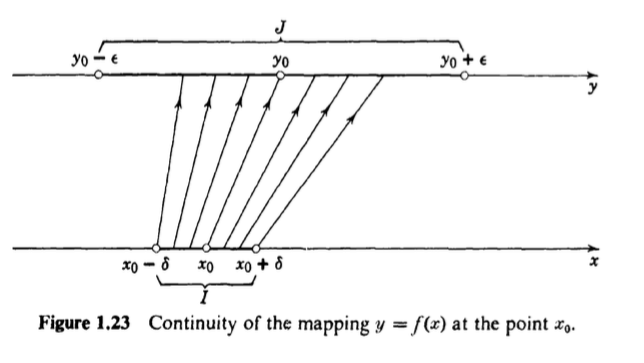
\includegraphics [scale=0.4] {continuity.png} \end{center}
In the figure above (from Courant and John), the mapping from $x$ to $y = f(x)$ is depicted generally using two number lines.  Below is a standard way of illustrating the same thing on the graph of $y=f(x)$.
\begin{center} 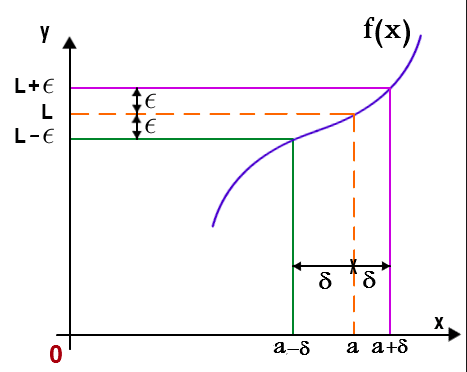
\includegraphics [scale=0.4] {continuity2.png} \end{center}

A particularly easy way to answer the question "is my function continuous at $x=a$" is to ask whether it is differentiable at $x=a$.  The reason is the following theorem:

\textcolor{blue}{If a function is differentiable at $x$, then it is continuous at $x$.}

Remember though, that continuity does \emph{not} imply differentiability.  A counterexample is the absolute value function at $x=0$.  The function is continuous, but the slope at $x=0$ does not exist (because the slopes coming in from the two directions are not the same).

\subsection*{funky functions}

Here are some examples:

\[ y = f(x) = \frac{x^2 (x-1)}{x-1} \]
This function acts just like $x^2$ except it has a "hole" in it at $x=1$, where it is undefined.  An exactly equivalent way to write it is

\[
f(x) =
\begin{cases}
x^2 & x \ne 1 \\
\text{undefined} & x = 1
\end{cases}
\]
We say that the limit of $f(x)$ as $x \rightarrow 1$ exists, because the one-sided limits $x \rightarrow 1^+$ and $x \rightarrow 1^-$ both exist \emph{and have the same value}.  It is not necessary for $f(x)$ to be defined at $x=a$ in order for the limit at $f(a)$ to be defined.

Another one is

\[ f(x) = \frac{1}{x^2} \]
This function is not defined at $x=0$

\subsection*{Jumps}

Functions can have jumps.  For example, let $f(x)$ be the greatest integer $\le x$.  So, for example, $f(\pi) = 3$.

\subsection*{One-sided limits not equal}

The function

\[ f(x) = \frac{1}{x} \]
is like $f(x)=1/x$, but it has an additional problem.  As $x$ becomes very close to zero from the right-hand side ($x \rightarrow 0^+$), $f(x)$ becomes infinitely large.  Whereas for $x \rightarrow 0^-$, the function becomes infinitely small.  Since these two one-sided limits are not equal, we say that the limit at $x=0$ does not exist.

\subsection*{Absolute value}

\[ f(x) = | x | \]

\subsection*{Gap}

\[ f(x) = \sqrt{x^2 - 16} \]
This function is simply not defined for $-4 < x < 4$.

\subsection*{Infinite oscillation}

\[ f(x) = \sin \frac{1}{x} \]
The value for $\sin x$ is always $-1 \le \sin x \le 1$, but as $x$ becomes smaller, $1/x$ becomes larger, and since every value of $1/x$ which is an integer multiple of $\pi$ has a sine of $0$ ($\sin n \pi = 0, n = 0, 1, 2 \dots$), the oscillations become faster and faster.

\subsection*{Mean Value Theorem}

A man passes a police car at point $A$ doing 60 mph (the speed limit) and 4 minutes later passes another police car at point $B$, also doing 60 mph, yet the second officer writes him a ticket for speeding, justified by the mean value theorem.  The reason:  point $A$ and point $B$ are 5 miles apart, hence the average speed over this interval was 75 mph, and \emph{must at least have been equaled at some point}.

If $f$ is a "nice" function on the interval $(a,b)$ then there exists at least one point $c$ in that interval where

\[ f'(c) = \frac{f(b) - f(a)}{b-a} \]

\begin{center} 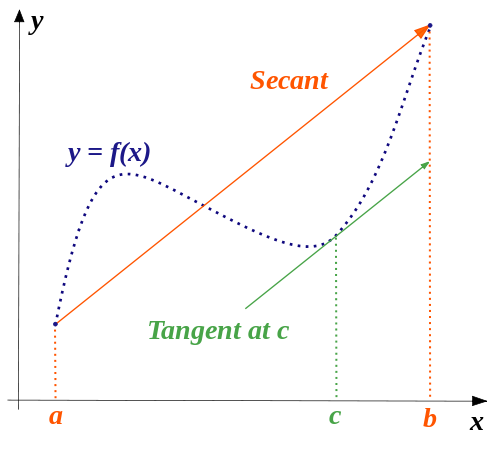
\includegraphics [scale=0.4] {mvt.png} \end{center}

What does it take to be "nice"?  The function $f$ must be continuous over the closed interval $[a,b]$ and differentiable over the open interval $(a,b)$.

The proof of the MVT relies on Rolle's Theorem, which is similar.  Rolle's Theorem says that for a "nice" $f$, if $f(a) = f(b)$, then there will exist at least one point $c$ in the interval $(a,b)$ such that $f'(c) = 0$.  The MVT proof basically turns Rolle's interval so that $a \ne b$.

\subsection*{Fundamental Theorem of Calculus}

\begin{center} 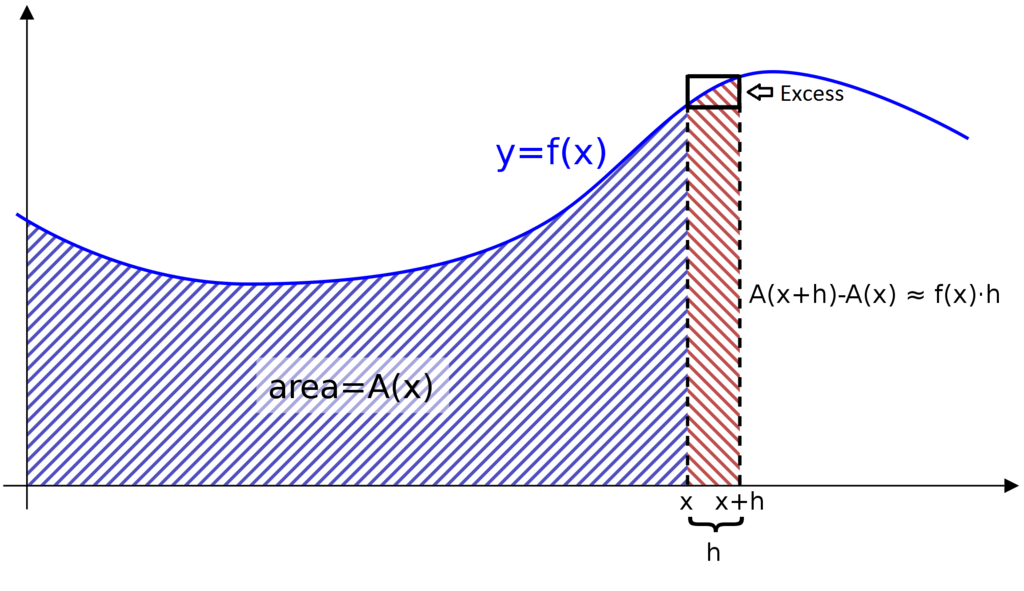
\includegraphics [scale=0.4] {FTC_geometric2.png} \end{center}

The big picture view of the fundamental theorem of calculus (FTC) is that if we consider that the area $A$ under the graph of a function $f(x)$ is itself a function $A(x)$ (having fixed the left-hand boundary for the area), then

\[ A' = f(x) \]

and we can find the area function $A$ as one of the family of \emph{anti-derivatives} of $f$.  

Now, there are conditions, namely that $F$ must be continuous on the interval $[a,b]$ and differentiable on $(a,b)$, and we agree to only look at $x$ values contained in the interval $(a,b)$.  In other words, the function $F$ and its derivative $f$ have to be "nice."  

There are two formal statements of the FTC, that turn out to be equivalent (the second can be proved from the first).

Suppose 
\[ F(x) = \int_a^x f(x) \ dx \]
then
\[ F'(x) = \frac{d}{dx} \ \int_a^x f(x) \ dx = f(x) \]

The expression $\int_a^x f(x) \ dx$ is a \emph{number}, a function of $x$, which gives a different result (usually) for each value of $x$.  Some people use the notation $f(t) \ dt$ so as not to be confused about this.  They will say

\[ F(x) = \int_a^x f(t) \ dt \]
\[ F'(x) = \frac{d}{dx} \ \int_a^x f(t) \ dt = f(x) \]

This is completely equivalent.

The area under the curve $y=f(x)$ betweeen a left-hand boundary $a$ and $x$ grows at the rate $f(x)$.  The derivative of the area function is $f(x)$.

The second version (FTC2) simply gives us a method to calculate what the number is, a way to evaluate integrals:

\[ \int_a^b f(x) \ dx = F(b) - F(a) \]

where $F$ and $f$ are the same as before, namely

\[ F'(x) = f(x) \]
If we can find a function $F$ whose derivative is equal to $f$ then we can evaluate the integral as shown.  An example:
\[ f(x) = x^2 \ dx \]
\[ F(x) = \frac{1}{3}x^3 \]
\[ \int_0^1 x^2 \ dx = \frac{1}{3}x^3 \ \bigg |_0^1 = \frac{1}{3}(1-0) = \frac{1}{3} \]
The area under the curve $f(x) = x^2$ between $x=0 \rightarrow 1$ is just $1/3$.

A simple-minded view of the FTC is that it says that integration and differentiation are the reverse processes for each other.  In fact, this is the fundamental insight of Newton and Leibnitz.

However, it is important to emphasize that the FTC is not the \emph{definition} of integration.  In fact, integration is defined as the limit of Riemann sums of the interval.  What the FTC does is to provide a way process that comes to the same answer as the sum method, but without the pain.

read Bressoud from p. 104 in the AP Calculus handout.









\end{document}  